
\documentclass[11pt,oneside]{book}

\usepackage[T1]{fontenc}
\usepackage[utf8]{inputenc}
\usepackage[margin=1in]{geometry}
\usepackage{hyperref}
\usepackage{longtable}
\usepackage{listings}
\usepackage{xcolor}
\usepackage{tikz}
\usetikzlibrary{arrows.meta,positioning,shapes.geometric}

\title{ROS 2 Engineering Handbook \\ Beginner to Advanced}
\author{Study Edition}
\date{\today}

\lstset{
basicstyle=\ttfamily\small,
breaklines=true,
frame=single
}

\begin{document}

\frontmatter
\maketitle
\tableofcontents

\chapter*{Preface}
This book provides a structured path from ROS 2 fundamentals to advanced
middleware, DDS, executors, lifecycle nodes, and production robotics systems.

\mainmatter

\part{Foundations}

\chapter{What is ROS 2?}

ROS 2 is a distributed robotics middleware framework built on DDS.

\section{Major Concepts}
\begin{itemize}
\item Nodes
\item Topics
\item Services
\item Actions
\item Parameters
\item DDS Middleware
\end{itemize}

\chapter{ROS 2 Architecture}

\section{Layered Architecture}

\begin{center}
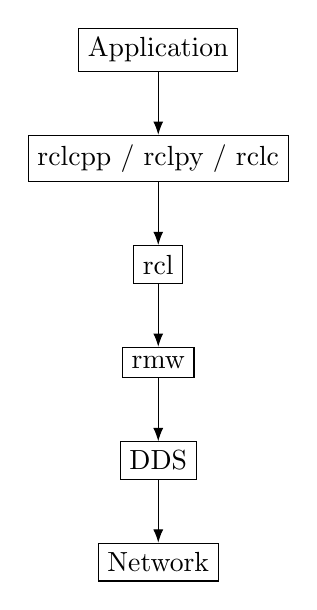
\begin{tikzpicture}[node distance=8mm]
\node[draw] (app) {Application};
\node[draw,below=of app] (rclcpp) {rclcpp / rclpy / rclc};
\node[draw,below=of rclcpp] (rcl) {rcl};
\node[draw,below=of rcl] (rmw) {rmw};
\node[draw,below=of rmw] (dds) {DDS};
\node[draw,below=of dds] (net) {Network};

\draw[-Latex] (app)--(rclcpp);
\draw[-Latex] (rclcpp)--(rcl);
\draw[-Latex] (rcl)--(rmw);
\draw[-Latex] (rmw)--(dds);
\draw[-Latex] (dds)--(net);
\end{tikzpicture}
\end{center}

\chapter{Workspace and Build System}

\section{Workspace Structure}

\begin{verbatim}
workspace/
 |-- src/
 |-- build/
 |-- install/
 `-- log/
\end{verbatim}

\section{Build}

\begin{lstlisting}[language=bash]
colcon build
source install/setup.bash
\end{lstlisting}

\part{Programming with ROS 2}

\chapter{C Development (rclc)}

\section{Embedded Architecture}

\begin{verbatim}
Application
   |
rclc
   |
rcl
   |
rmw
   |
DDS
\end{verbatim}

\chapter{C++ Development (rclcpp)}

\section{Publisher Example}

\begin{lstlisting}[language=C++]
class Talker : public rclcpp::Node
{
public:
  Talker() : Node("talker")
  {
    publisher_ =
      create_publisher<std_msgs::msg::String>(
      "chatter",10);
  }
};
\end{lstlisting}

\chapter{Python Development (rclpy)}

\section{Publisher Example}

\begin{lstlisting}[language=Python]
class Talker(Node):

    def __init__(self):
        super().__init__("talker")

        self.pub = self.create_publisher(
            String,
            "chatter",
            10
        )
\end{lstlisting}

\part{Communication}

\chapter{Topics}

\begin{center}

\begin{tikzpicture}[node distance=3cm]
\node[draw] (pub) {Publisher};
\node[draw,right=of pub] (topic) {Topic};
\node[draw,right=of topic] (sub) {Subscriber};

\draw[-Latex] (pub)--(topic);
\draw[-Latex] (topic)--(sub);
\end{tikzpicture}
\end{center}

\chapter{Services}

\begin{verbatim}
Client --> Request
Server --> Response
\end{verbatim}

\chapter{Actions}

\begin{verbatim}
Goal
 |
Feedback
 |
Result
\end{verbatim}

\chapter{QoS}

\begin{longtable}{|p{2in}|p{3in}|}
\hline
Policy & Description \\ \hline
Reliability & Reliable / Best Effort \\ \hline
Durability & Message persistence \\ \hline
History & Queue depth \\ \hline
Deadline & Timing guarantees \\ \hline
\end{longtable}

\part{DDS Deep Dive}

\chapter{DDS Entities}

\begin{itemize}
\item Domain Participant
\item Publisher
\item Subscriber
\item DataWriter
\item DataReader
\end{itemize}

\chapter{Discovery}

\begin{center}

\begin{tikzpicture}[node distance=4cm]
\node[draw] (p) {Publisher};
\node[draw,right=of p] (s) {Subscriber};

\draw[-Latex] (p) -- node[above]{Discovery Traffic} (s);
\draw[-Latex] (s) -- node[below]{Match} (p);
\end{tikzpicture}
\end{center}

\part{Talker and Listener Internals}

\chapter{Process Creation}

Command:

\begin{lstlisting}[language=bash]
ros2 run demo_nodes_cpp talker
\end{lstlisting}

Operating system creates:

\begin{verbatim}
PID 1001
Talker Process
\end{verbatim}

\chapter{Message Journey}

\begin{center}
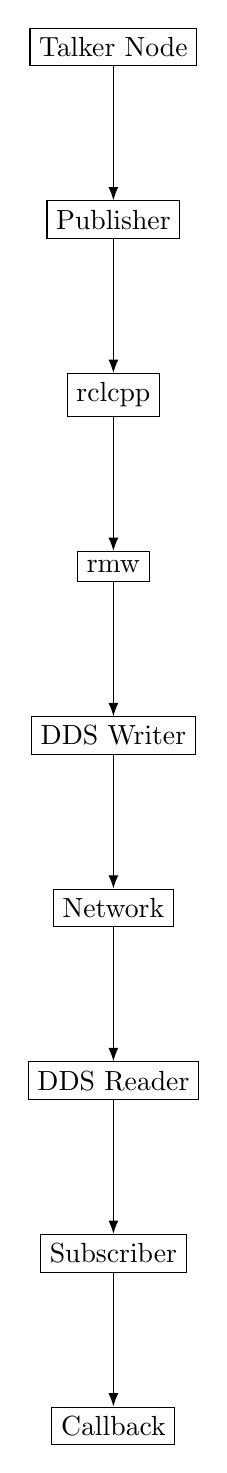
\begin{tikzpicture}[node distance=1.7cm]
\node[draw] (a) {Talker Node};
\node[draw,below=of a] (b) {Publisher};
\node[draw,below=of b] (c) {rclcpp};
\node[draw,below=of c] (d) {rmw};
\node[draw,below=of d] (e) {DDS Writer};
\node[draw,below=of e] (f) {Network};
\node[draw,below=of f] (g) {DDS Reader};
\node[draw,below=of g] (h) {Subscriber};
\node[draw,below=of h] (i) {Callback};

\draw[-Latex] (a)--(b);
\draw[-Latex] (b)--(c);
\draw[-Latex] (c)--(d);
\draw[-Latex] (d)--(e);
\draw[-Latex] (e)--(f);
\draw[-Latex] (f)--(g);
\draw[-Latex] (g)--(h);
\draw[-Latex] (h)--(i);
\end{tikzpicture}
\end{center}

\section{Detailed Flow}

\begin{enumerate}
\item OS creates process.
\item ROS initializes.
\item Node created.
\item Publisher created.
\item DDS participant created.
\item Discovery begins.
\item Subscriber matches topic.
\item Message serialized.
\item DDS transmits bytes.
\item Subscriber receives bytes.
\item Message deserialized.
\item Executor schedules callback.
\item User callback executes.
\end{enumerate}

\chapter{Executors}

\section{Single Threaded}

\begin{lstlisting}[language=C++]
rclcpp::spin(node);
\end{lstlisting}

Responsibilities:

\begin{itemize}
\item Wait for DDS events
\item Execute callbacks
\item Process timers
\item Handle services and actions
\end{itemize}

\part{Advanced ROS 2}

\chapter{Lifecycle Nodes}

\begin{verbatim}
Unconfigured
    |
Configured
    |
Active
    |
Inactive
    |
Finalized
\end{verbatim}

\chapter{Composition}

Multiple nodes can run inside a single process.

Benefits:

\begin{itemize}
\item Less memory
\item Faster communication
\item Reduced context switching
\end{itemize}

\chapter{Real-Time ROS 2}

Topics:

\begin{itemize}
\item Deterministic scheduling
\item Memory pre-allocation
\item Lock-free structures
\item Real-time executors
\end{itemize}

\chapter{Security}

SROS2 provides:

\begin{itemize}
\item Authentication
\item Encryption
\item Access control
\end{itemize}

\part{Robot Systems}

\chapter{Navigation Stack}

\begin{verbatim}
Map
 |
Localization
 |
Planning
 |
Controller
 |
Robot
\end{verbatim}

\chapter{Perception}

Camera, LiDAR, IMU and sensor fusion systems.

\chapter{Manipulation}

MoveIt 2 architecture and robot arm planning.

\part{Projects}

\chapter{Suggested Projects}

\begin{enumerate}
\item Differential drive robot
\item SLAM robot
\item Warehouse robot
\item Multi-robot fleet
\item Autonomous rover
\end{enumerate}

\backmatter

\chapter{Further Reading}

Official ROS 2 documentation, Navigation2, MoveIt 2, Gazebo and Micro-ROS.

\end{document}
